\documentclass[../dejiny-rodu-prusiku.tex]{subfiles}

\begin{document}


% str 52 @ 65
\section{O dobrodinci rodu, knězi Blažejovi Prusíkovi}

Jako třetí dítě Vojtěcha Prusíka a jeho ženy Anny, roz. Fenclové ve Výrově, narodil se 1. února 1810 první jejich syn. Při křtu v Kralovicích dostal jméno po svém dědovi Blažejovi, který žil tehdy již na výměnku jako osmašedesátiletý v Sedlci. Tento Blažej Prusík, který se stal později knězem, zaujímá  zvláštní postavení v dějinách našeho rodu. Otec jeho, výrovský rychtář, Vojtěch Prusík dal svého prvorozeného syna na studie. Přáním rodičů bylo, aby se stal knězem. Ti byli vedle učitelů v té době předvojem inteligence v národě a zásluhou mno­hých uvědomělých českých kněží vniklo do našeho lidu ne­jen národní uvědomění, ale i hospodářský pokrok, zvlášť v zemědělství. Podobnou úlohu sehrál v dějinách výrovské větve rodu Prusíků Blažej Prusík. Je plným právem pojmenován v našem rodě jako "dobrodinec“.

Po studiích v Praze byl Blažej vysvěcen na kněze 6. srpna 1837. Bylo to za panování císaře Ferdinanda Dobrotivého. 1. prosince 1837 nastoupil Blažej jako kaplan do Dobříše, kde působil do 15. července 1841. To byla ještě doba roboty. Odtud dostal se do Prahy a dalším jeho působištěm byl kostel u sv. Mikuláše na Malé Straně. Toto místo bývalo velmi často přestupní stanicí pro další vyšší povolání. A skutečně i Blažej Prusík odešel v roce 1850 odtud na Hradčany ke sv. Vítu. Stal se tam průběhem let vikářem, arcibiskupským notářem, ceremoniářem liturgie a později i zpovědníkem tehdejšího Tereziánského ústavu šlechtičen na Hradčanech. Do té doby, než byl zpovědníkem měl ročně 800 zlatých. Ani potom, když zlepšil své hmotné postavení o 400 zlatých ročně, není možno tvrdit o něm, že to byl bohatý kněz. Jistě by 100 zlatých měsíčně utratil se svou hospodyní snadno sám. Blažej bydlil těsně u svatovítské katedrály vedle nynější restaurace Vikárky, kterou tak nezapomenutelně zvěčnil básník Svatopluk Čech svým „Výletem pana Broučka do XIV. století". Dům, kde Blažej léta bydlil a prokazoval dobrodiní, má číslo 8 a kdokoliv ze členů rodu našeho jde kolem při návštěvě Hradu, může si na tohoto šlechetného člověka s láskou vzpomenout.

U vikáře Blažeje bydlili postupem let a v Praze studova­li četní Prusíci. I když jejich otcové dovezli pro své děti ty nejnutnější potraviny jednou za rok povozem, více již nemohli věnovati na výchovu svých dětí. Doma  měli rodiny početné a tak pro ně jejich bratr, kněz Blažej byl opravdovou spásou, když chtěli, aby jejich děti vystudovaly.

Do Prahy jezdil tedy ročně Tomáš Prusík z Horní Břízy, Matěj z Hodyně a Václav z Výrova a dovezli svým dětem k bratrovi do Prahy to nejnutnější. Jezdilo se tehdy přes velké lesy. Leckdy nebylo v nich bezpečno. Teprve od roku

% str 53 @ 66
1861 nastal velký pokrok, kdy se počalo cestovat dostavníkem. Pak mohli i synovci vikáře Blažeje jako studenti používati tohoto dopravního prostředku. V Praze u svého strýčka studoval jako první Jan Prusík z Horní Břízy. Později tam byl jeho bratr Tomáš, kte­rý se stal knězem. Z Hodyně byl to synovec vikářův František a Jan, kteří sice nestudovali na universi­tě, ale přece jen nižší studium jim pomohlo k pozděj­ší lepší existenci. Z výrovské usedlosti přišli k Blažejovi v průběhu let dokonce čtyři jeho synovci. Nejdříve tam byl Blažej, který se stal později profesorem, dále jeho bratr František, pozdější známý slavista, Václav, který byl magistrátním úředníkem v Pra­ze a nejmladší Josef, který také díky podpoře svého strýce, domohl se pak slušné existence.

Vikář Blažej Prusík působil 35 let na Hradčanech za arcibiskupa Bedřicha Schwarzenberka a ještě pak tři léta za arcibiskupa Františka Schőnborna. Byl z vikářů jako jediný Čech.

Že úkol, který na sebe vzal Blažej Prusík, nebyl snadný vidíme i z upřímného doznání v jednom dopise, který píše do Klatov svému synovci Blažejovi, mladému profesorovi. Bylo to 28. října 1871. Píše mimo jiné: "Všecko jsem ti tedy zevrubně vypsal a z toho vidíš, jak velké břímě já letos na sobě mám. S Janem jest nás 9 osob, Tomáš v semináři také ledacos potřebuje, z domova jemu téměř nic dáti nemohou, kam se tedy má obrátit než ke mně, když něco potřebuje. Zajisté jest to div, že já přece tak vycházím. Jak jsi o té velké láci v Klatovech psal, divili jsme se tomu  všichni a pravili, že nejméně ještě jednou tolik všecky ty věci zde v Praze stojí. Dříví jest tam u Vás také poměrně laciné, kup  si na zimu buď březové nebo habrové a sice hezky mnoho, neboť budeme mít letos zase velmi krutou zimu. Buď dobře zdráv a v ochranu Boží Tebe poroučeje zůstávám vždy Tvůj upřímný strejček, Blažej Prusík."

Osm synovců Blažejových děkuje tedy za mnoho dobra. Nepřímo jsou to však i další jejich potomci. Ve vzpomínkové knížce o svém výrovském rodu opravdu správně připomíná všem dalším generacím Prusíků jeden z vystudovaných synovců u vikáře Blažeje, Josef. Napsal toto: „Vy všichni, kteří toto čtete, byli jste a jste přímým i nepřímým způsobem účastni jeho dobrodiní. A nikdy toho nezapomeňte. Nebýti jeho, nebylo by studií synů, neprovdaly by se bývaly tak dobře dcery, nýbrž by se byl rodný statek rozpadl na mnoho drobných dílů. Ze synů stali by se chalupníci a malí řemeslníci a jméno jejich a dílo by bylo sotva proniklo do veřejnosti. Proto Blažej Prusík, vikář na Hradčanech má lví podíl na lepší existenci celého rodu Prusíků, který vzešel z jedné větvi z Výrova.

Vikář Blažej nepodporoval však jen své synovce, studenty. Svou vzdělaností a přehledem o hospodářském pokroku ve světě, k němuž měl v Praze dobrý přístup, pomáhal cennými radami i materiálně v modernějším hospodaření

% str 54 @ 67
svých bratří, sedláků. Že jako první začal používat kosy při žních jeho bratr Václav ve Výrově, či nových strojů tam v Hodyni i Horní Bříze, je jeho nepřímou zásluhou. I ovocné stromy dával zasílati domů do Výrova i jinam a tak pomáhal zkrášlovat svůj rodný kraj. Sám byl neobyčejně skromný. Jen o svátcích přišel na stůl jeden litr piva, pod klerikou nosil celou řadu let koženky, které si sám spravoval. Velice se zlobil, když mu jednou k svátku koupili nové koženky. Všechno, co měl, věnoval na své svěřence a když mohl ještě něco bratrům při návštěvě v Praze, daroval.

Blažej chystal se ke konci svého života odstěhovati se svou hospodyní na Staré město do  blízkosti bytu, kde byl usazen jeho synovec profesor F. X. Prusík. Dříve však než k tomu došlo, zemřel. Zápal plic ukončil jeho záslužný život dne 22. srpna 1888. Byl pochován na hřbitově u sv. Markéty v Břevnově. Od těch dob je stále jeho hrob vyplácen a udržován na jeho věčnou paměť. Leží blízko hromadného hrobu břevnovských řeholníků a u jeho hrobu měli by se zastavit členové našeho rodu a vzpomenout, co vlastně i pro ně vykonal.

Do sbírky svých básní napsal vděčný synovec ušlechtilého kněze Blažeje, Josef Prusík tuto elegii:

\settowidth{\versewidth}{a duma - list, jenž uschlý, hrob Tvůj kryje?}
\begin{verse}[\versewidth]
Zde ležíš tedy - zde Tvá rakev hnije, \\
kde smutná vrba nad hrobem se sklání, \\
kde tichý větřík dumy popohání - \\
a duma - list, jenž uschlý, hrob Tvůj kryje? \\
Jen duše Tvá snad na nás dolů hledí, \\
jak pro Tebe tu synovci my lkáme \\
a Tebe z hrobu temna voláváme - \\
leč modrý ret v útěchu slova neví. \\
Spi dobrodinče náš ve hrobu stíně \\
za život přejem věčné Tobě slasti, \\
že jím‘s nám dával příklad lásky k vlasti \\
a nové budil syny domovině. \\
Zde ležíš,  strýče, tu že dřímáš tedy, \\
kde smutná vrba dumkou dlouhou šumí- \\
ó spi jen, spi - můj duch Ti porozumí, \\
a vykoná, cos šept mně naposledy.
\end{verse}

Napsáno 13. prosince 1890.

% str 54+1 @ 68
\begin{figure}
\centering
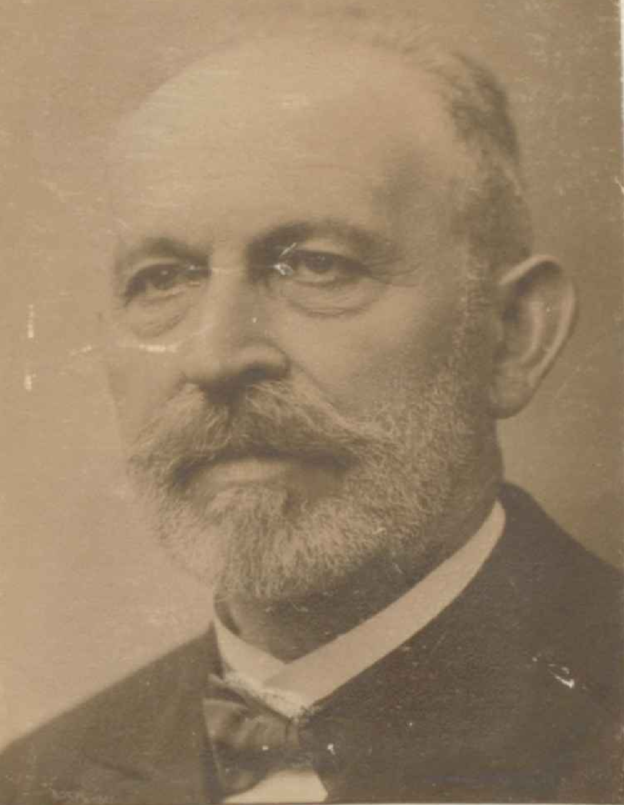
\includegraphics[width=\textwidth, height=\textheight, keepaspectratio]{068-a-profesor_blazej_prusik}
\caption{Prof. Blažej Prusík, rodák z Výrova (1844 – 1912), učitel J. Thomayera a J. Vrchlického na klatovském gymnáziu}
\label{fig:068-a-profesor_blazej_prusik}
\end{figure}

\begin{figure}
\centering
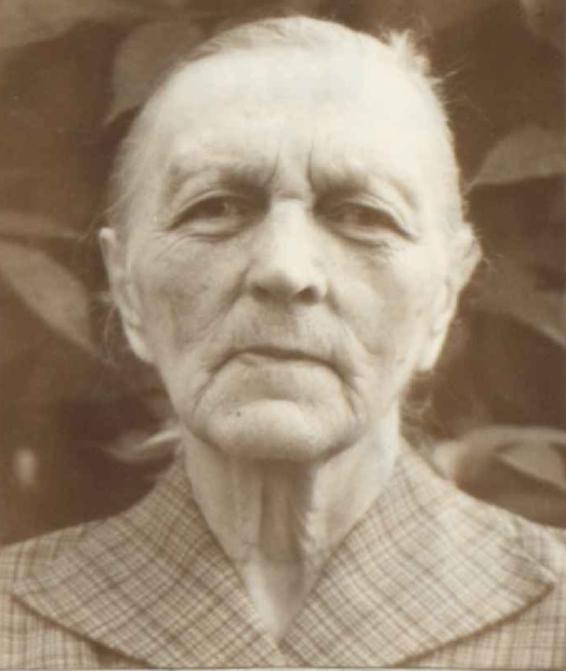
\includegraphics[width=\textwidth, height=\textheight, keepaspectratio]{068-b-anna_meixnerova}
\caption{Anna Meixnerová roz. Prusíková z Výrova (1886 – 1967). Po zakladateli větve Vojtěchu Prusíkovi, zemřelém roku 1841 ve Výrově, je ona posledním členem rodu}
\label{fig:068-b-anna_meixnerova}
\end{figure}

\begin{figure}
\centering
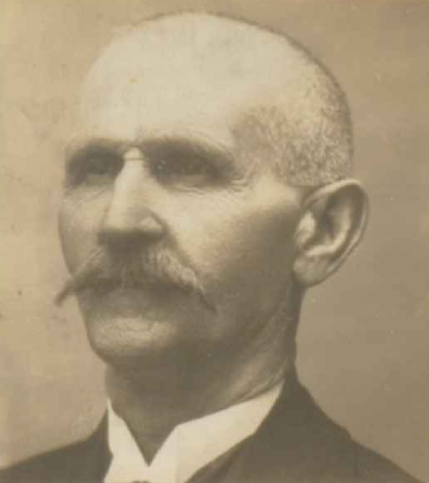
\includegraphics[width=\textwidth, height=\textheight, keepaspectratio]{068-c-vojtech_prusik_z_hodyne}
\caption{Vojtěch Prusík rodák z Hodyně (1847 – 1924), dlouholetý starosta a průkopník moderního zemědělství}
\label{fig:068-c-vojtech_prusik_z_hodyne}
\end{figure}

\begin{figure}
\centering
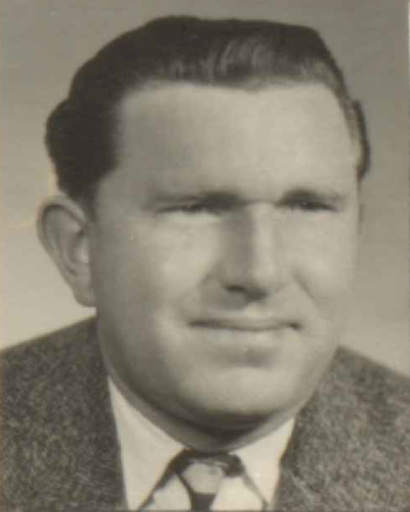
\includegraphics[width=\textwidth, height=\textheight, keepaspectratio]{068-d-ing_ladislav_prusik}
\caption{Ing. Ladislav Prusík z Horní Břízy je posledním Prusíkem, který žije v sídle tří zakladatelů odnože větve Výrov}
\label{fig:068-d-ing_ladislav_prusik}
\end{figure}

 \begin{figure}
\centering
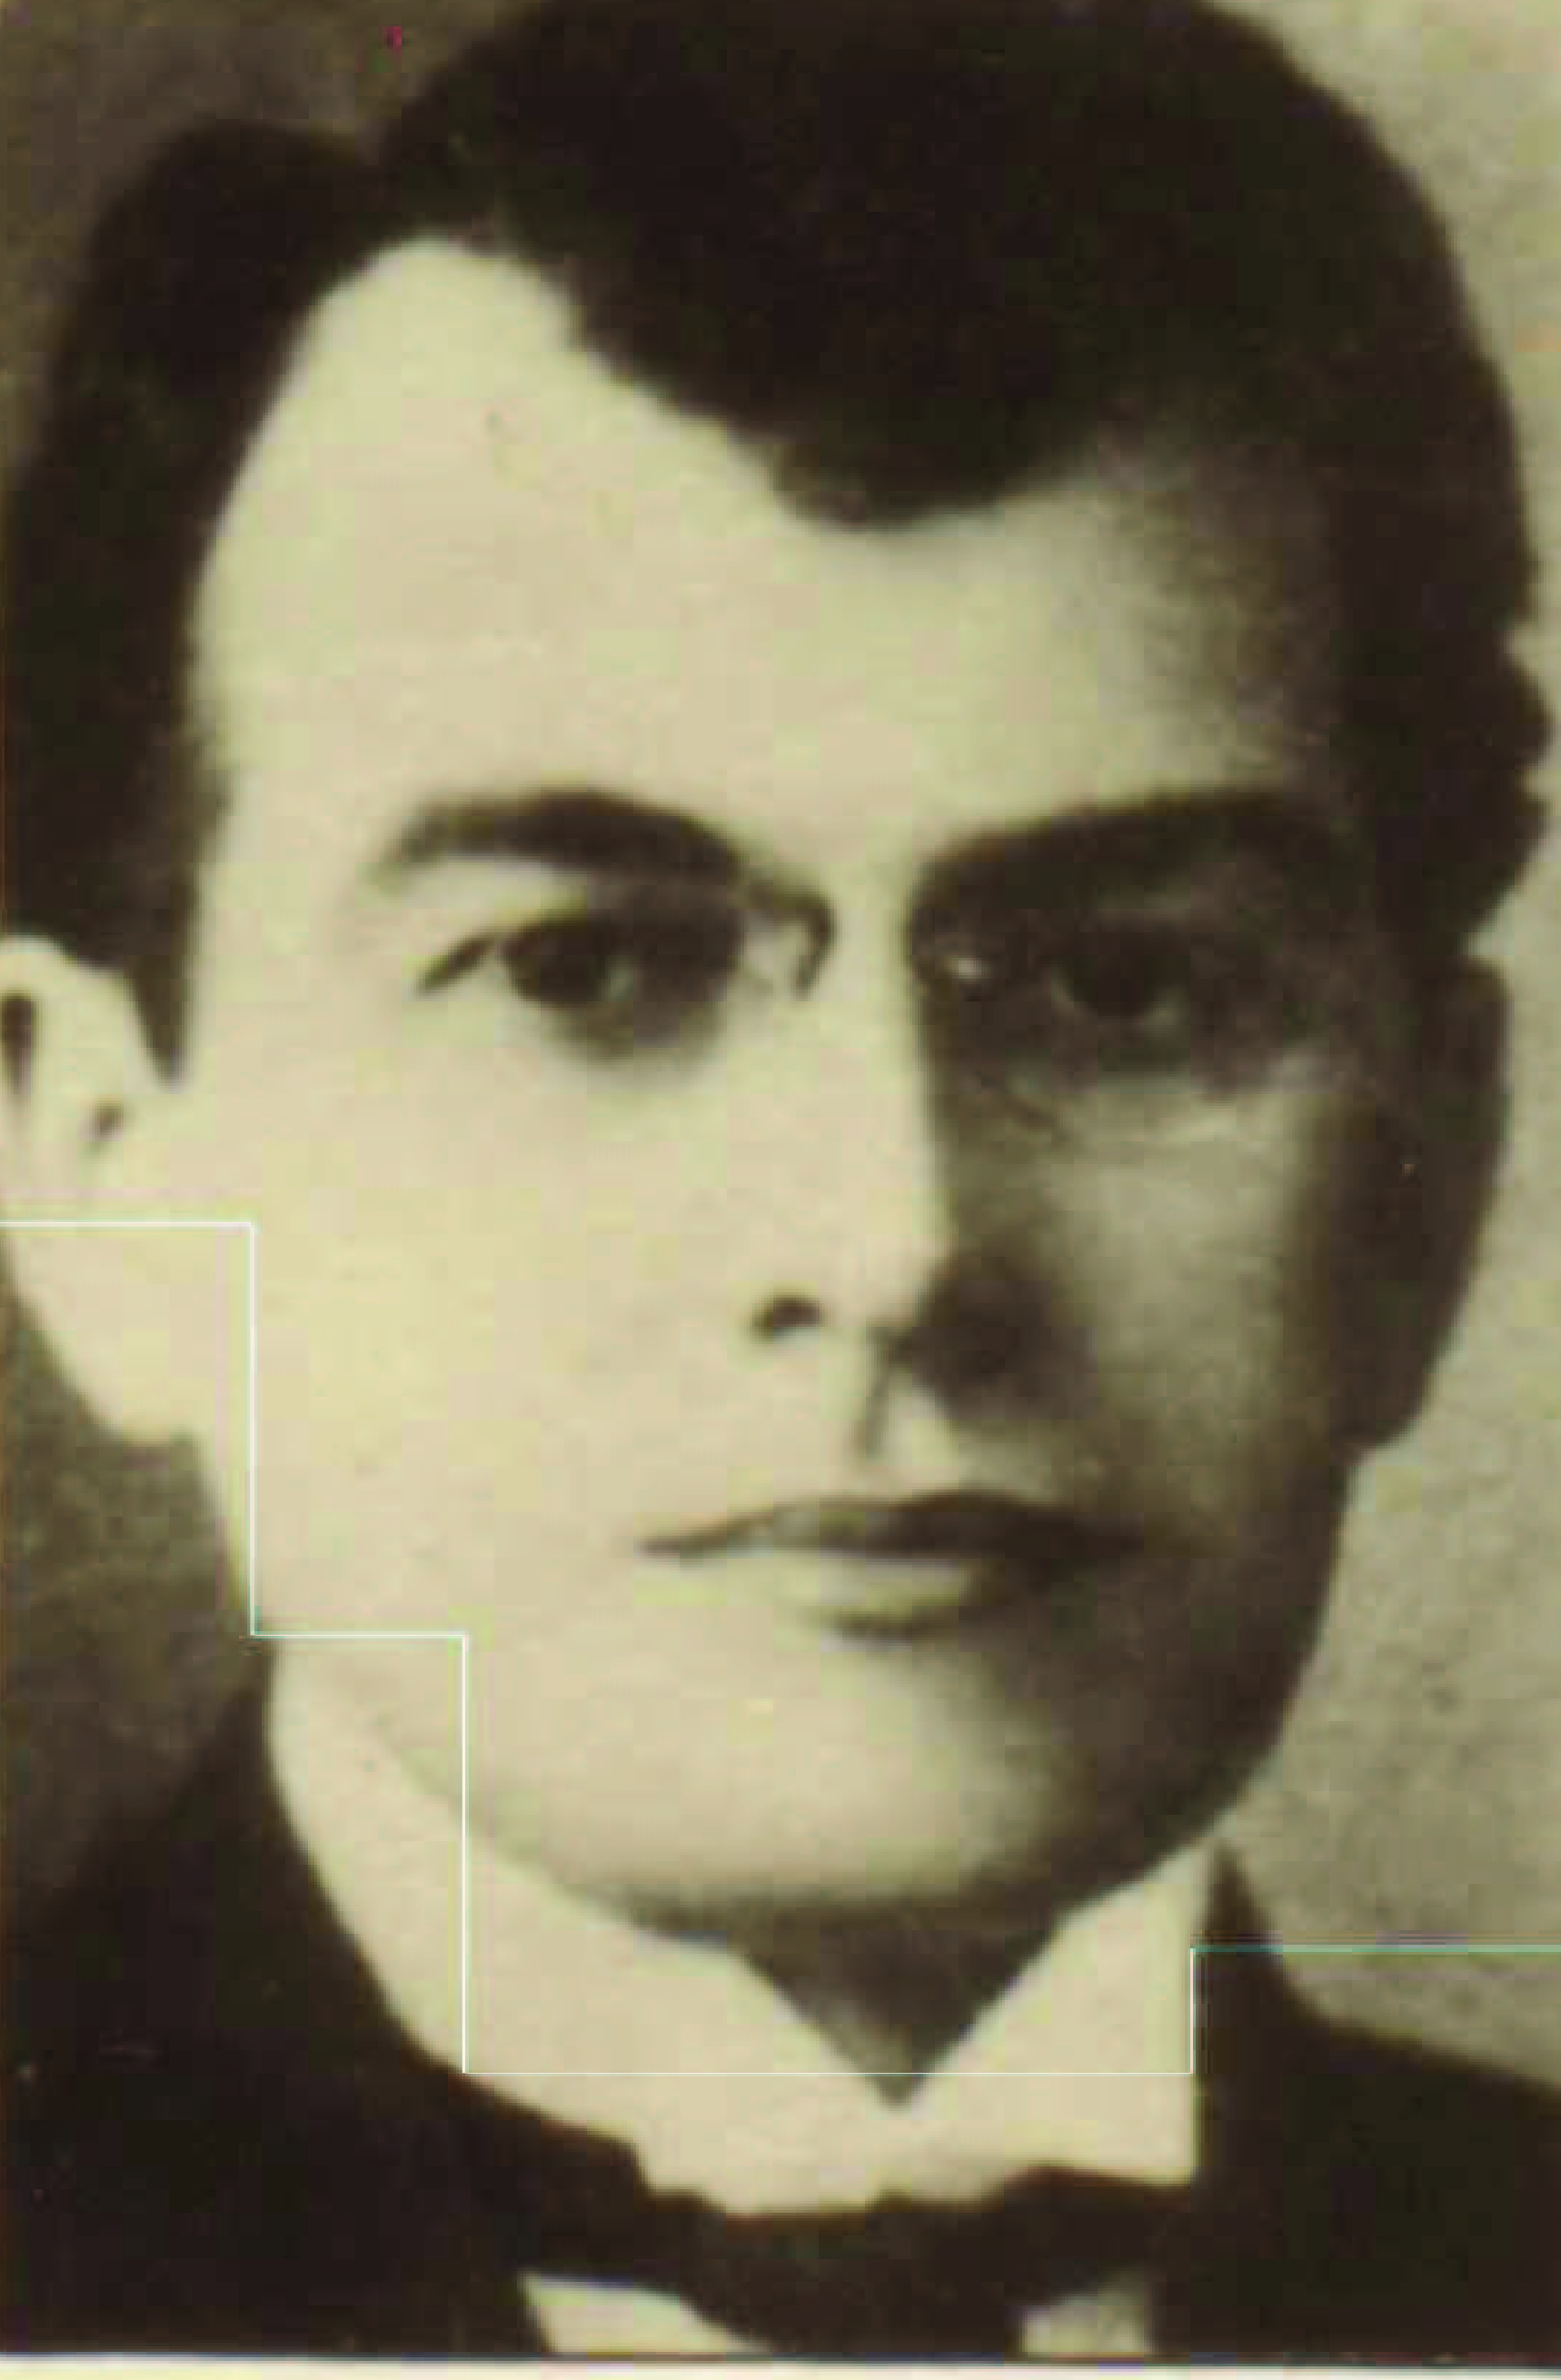
\includegraphics[width=\textwidth, height=\textheight, keepaspectratio]{068-e-robert_prusik}
\caption{Robert Prusík, rodák z Luže (1878 – 1937), zcestoval ze všech Prusíků největší kus světa}
\label{fig:068-e-robert_prusik}
\end{figure}

\end{document}
